\documentclass[a4paper,10pt,fleqn, twocolumn]{IEEETran}
\usepackage{amsfonts}
\usepackage{amsthm}
\usepackage{graphicx}
\usepackage{fancyhdr}

\setlength{\parindent}{3em}
\setlength{\oddsidemargin}{0in}
\setlength{\textwidth}{6.5in} % sets 1in left and right margins
\setlength{\topmargin}{0.0in} % change to 0.2in for regular latex
%\setlength{\headheight}{0in}
%\setlength{\footheight}{0.5in}
\setlength{\footskip}{0.5in}
\setlength{\textheight}{9.0in} %sets 1in top and bottom margins
%\renewcommand{\baselinestretch}{1} %set to 1.5 for double spacing.


\newtheorem{Prop}{Proposition}
\newtheorem{lemma}{Lemma}

\newcommand{\br}{{\mathbf r}}
\newcommand{\bA}{{\mathbf A}}
\newcommand{\ba}{{\bf a}}
\newcommand{\bb}{{\bf b}}
\newcommand{\bc}{{\bf c}}
\newcommand{\bC}{{\bf C}}
\newcommand{\bd}{{\bf d}}
\newcommand{\bg}{{\bf g}}
\newcommand{\bG}{{\bf G}}
\newcommand{\be}{{\bf e}}
\newcommand{\bs}{{\bf s}}
\newcommand{\bm}{{\bf m}}
\newcommand{\bn}{{\bf n}}
\newcommand{\bu}{{\bf u}}
\newcommand{\bv}{{\bf v}}
\newcommand{\bw}{{\bf w}}
\newcommand{\bx}{{\bf x}}
\newcommand{\by}{{\bf y}}
\newcommand{\bbf}{{\bf d}}
\newcommand{\bE}{{\bf E}}
\newcommand{\bF}{{\bf F}}
\newcommand{\bL}{{\bf L}}
\newcommand{\bM}{{\bf M}}
\newcommand{\bN}{{\bf N}}
\newcommand{\bS}{{\bf S}}
\newcommand{\bT}{{\bf T}}
\newcommand{\bD}{{\bf D}}
\newcommand{\bX}{{\bf X}}
\newcommand{\bP}{{\bf P}}
\newcommand{\bQ}{{\bf Q}}
\newcommand{\bI}{{\bf I}}
\newcommand{\bR}{{\bf R}}
\newcommand{\bU}{{\bf U}}
\newcommand{\bV}{{\bf V}}
\newcommand{\bW}{{\bf W}}
\newcommand{\bJ}{{\bf J}}
\newcommand{\bB}{{\bf B}}
\newcommand{\bzero}{{\bf 0}}
\newcommand{\bgamma}{{\mbox {\boldmath $\gamma$}}}
\newcommand{\btheta}{{\mbox {\boldmath $\theta$}}}
\newcommand{\bLambda}{{\mbox {\boldmath $\Lambda$}}}
\newcommand{\bPsi}{{\mbox {\boldmath $\Psi$}}}
\newcommand{\bPhi}{{\mbox {\boldmath $\Phi$}}}
\newcommand{\bcA}{{\mbox {\boldmath ${\cal A}$}}}
\newcommand{\bcB}{{\mbox {\boldmath ${\cal B}$}}}
\newcommand{\bcC}{{\mbox {\boldmath ${\cal C}$}}}
\newcommand{\bcD}{{\mbox {\boldmath ${\cal D}$}}}
\newcommand{\bcF}{{\mbox {\boldmath ${\cal F}$}}}
\newcommand{\bcN}{{\mbox {\boldmath ${\cal N}$}}}
\newcommand{\bcS}{{\mbox {\boldmath ${\cal S}$}}}
\newcommand{\bcH}{{\mbox {\boldmath ${\cal H}$}}}
\newcommand{\bcI}{{\mbox {\boldmath ${\cal I}$}}}
\newcommand{\bcR}{{\mbox {\boldmath ${\cal R}$}}}

\title{ Semi-Blind Adaptive Multiuser Detection For Asynchronous CDMA }
\date{}
\author{Shu Wang, Sang G. Kim, James Caffery, Jr., Li-Hsiang Sun, Hobin Kim,\\Suk W. Lee, S. R. Subramanya, Ki Y. Kim and Byung K. Yi}
\begin{document}
\maketitle
\begin{abstract}\small
In this paper, we propose a semiblind multiuser detection
framework for asynchronous CDMA. Compared with most existing
semiblind/blind detectors, the proposed framework requires a
minimum number of previously received signals, which is about the
number of interfering signals, and no detection filter converging
or subspace separation procedure. The computational complexity and
detection delay are therefore much lower. In this framework, a
semiblind multiuser signal model is used instead of the
widely-discussed conventional multiuser model or subspace-based
parametric multiuser signal model. Following this framework,
several semiblind linear detectors are developed using least
squares (LS), minimum variance unbiased estimation (MVU) and
minimum mean squared error (MMSE) estimation criteria. Meanwhile,
a multi-window scheme is proposed for simultaneously detecting
several bits and a recursively adaptive procedure is developed for
further lowering the complexity. After these, the asymptotic
multiuser efficiency (AME) of the proposed framework, the
comparison between the employed semiblind multiuser signal model
and the conventional signal model, and several estimation bounds
are discussed. Computer simulation results are presented to
support the performance of the proposed semi-blind multiuser
detection schemes.
\end{abstract}
\section{Introduction}
Multiuser detection strategy is a method for minimizing the effect
of multiple access interference (MAI) and solving the near-far
problem without a significant reduction in the signal energies of
the strong users in order for the weaker users to achieve reliable
communication. It has been extensively investigated over the past
decades or so, since MAI is the dominant impairment for CDMA
systems and exists even in perfect power-controlled CDMA
systems~\cite{Verd86,Verd89,Lupa89,Madh94,Honi95,Wang98,Verd98,Wang99}.
Most multiuser detection schemes are based on the conventional
multiuser signal model and then detect desired users' bits using
statistical signal estimation techniques, which include the
minimum bit-error rate (MBER)~\cite{Verd86,Verd89}, least-square
errors~\cite{Lupa89}, MMSE~\cite{Lupa89,Madh94,Honi95} and minimum
output energy (MOE)~\cite{Honi95} criteria. In the conventional
signal model, received signals and multiuser receivers are
represented by using users' amplitudes, timing and spreading
signatures, which are difficult to be known a prior by most
semiblind/blind detectors. On the other hand, the converging and
training procedure employed by many semiblind/blind multiuser
detectors for discovering interference structure normally cost
multiuser receivers lots of time and computation resources.
Recently, there have been lots of attentions focused on
subspace-based signal models, in which each received signal is
taken as a combination of the bases of signal and noise
subspaces~\cite{Yang95,Liu96,Torl97}, and subspace-based multiuser
detectors~\cite{Wang98,Wang99}. Subspace-based multiuser detection
essentially is a method for blindly reconstructing existing
conventional detectors. Although their performance can be well
above many previous semiblind/blind approaches, subspace-based
multiuser detectors need compute the covariance matrix of received
signals and separate signal/noise subspace bases. This makes it
difficult to be implemented in many practical situations,
especially where the wireless channel and the number of users
experience fast dynamic changes. Hence, recent blind multiuser
detection research is focused on reducing detection complexity and
delay.

Although both the conventional multiuser signal model and
subspace-based multiuser signal model provide a natural and
straightforward description of received signals, most semiblind or
blind detectors based on them are hard to be implemented in many
practical applications since the signal bases used in these two
models are unknown beforehand and it is nontrivial to estimate
them by receivers. In order to detect desired user's information
bits with minimum computational complexity and prior knowledge, we
propose a semiblind multiuser signal model and a novel multiuser
detection framework, which require only desired users' spreading
sequence, amplitude, several previously received signals and
possible channel noise variance, for asynchronous CDMA channel.
Based on this framework, we develop several semiblind linear
multiuser detectors using least squares, minimum variance unbiased
and minimum mean squared estimation criteria. In the proposed
signal model and framework, each received asynchronous signal and
semiblind receiver is taken as a combination of the desired user's
spreading sequence, several previously received signals and noise.
Therefore, there is no detection filter convergence or subspace
separation procedure required for interference signal structure
discovery. The proposed semiblind schemes are simple and direct.
They require a minimum number of previously received signals,
which is about the number of interfering signals. A recursively
adaptive implementation is developed for further reducing the
complexity. Finallt, the comparison between the proposed semiblind
signal model and the conventional model, the asymptotic multiuser
efficiency of the proposed framework, several estimation bounds
and also computer simulations are presented to demonstrate their
performance.
\section{Data Model and Problem Description}
The conventional $K$-user asynchronous multiuser model is
presented~\cite{Verd98}. The baseband representation of the
received signal due to the $k$th user is given by
\begin{equation}
\begin{array}{rcl}
r_k(t)&=&\sum\limits_{i=-\infty}^{+\infty}A_k b_k[i]
s_k(t-iT_c-\tau_k)
\end{array}
\end{equation}
\noindent where $b_k[i]$ is the $i$th bit sent by the $k$th user.
We assume that $\left\{b_k[i]\right\}$ are independent and
identically distributed random variables with ${\rm
E}\left\{b_k[i]\right\}=0$ and ${\rm
E}\left\{|b_k[i]|^2\right\}=1$. $s_k(t)$ denotes the normalized
signal waveform of the $k$th user during the interval $[(n-1)T,\
nT]$, $\tau_k\in[0,\ T_c)$ is a uniform random variable which
denotes the transmission delay from the $k$th user to the base
station and $A_k$ is the amplitude of the received signal of the
$k$th user. The baseband signal at the input of the receiver at
the mobile station is
\begin{equation}
\begin{array}{rcl}
r(t)&=&\sum\limits_{k=1}^{K}r_k(t)+n(t)
\end{array}
\end{equation}
\noindent where $n(t)$ is additive white Gaussian noise (AWGN)
with power spectral density $\sigma_n^2$.

The received signal is synchronized for each user individually,
passed through the corresponding chip matched filter (CMF) and
sampled at least at the chip rate $1/T_c$. The vector of the
output samples of the CMF for $k$th user in the $n$th symbol
interval can be expressed as
\begin{equation}\hspace{-0.1in}
\begin{array}{l}
\br_k{[n]}=\left[
\matrix{r_k(nT+T_c+\tau_k)&\ldots&r_k(nT+LT_c+\tau_k)}\right]^{\rm
T}\ .
\end{array}
\end{equation}
\noindent where $L$ denotes the spreading gain.

Prior to developing our semi-blind decorrelating detectors, we
review the classic single-truncated-window decorrelating detector,
in which the system is assumed to be chip-synchronous and the
observation window is restricted to one symbol
interval~\cite{Verd98}. Without loss of generality, we consider
the detection of the first user while the other users' signals are
treated as interference. A typical interferer has two consecutive
symbols interfering with the symbol of user $1$ so that the
received signal $\br$ can be conventionally and straightforwardly
expressed by
\begin{equation}\hspace{-0.1in}
\begin{array}{rcl}
\br_1&\hspace{-0.1in}=&\hspace{-0.1in}A_1b_1{[n]}\bs_1+\sum\limits_{\tau_k\geq\tau_1}^{K}A_k\left\{b_k{[n-1]}
\bs_{k-}+b_k{[n]} \bs_{k+}\right\}\\
&&+\sum\limits_{\tau_k<\tau_1}^{}A_k\left\{b_k{[n]}
\bs_{k-}+b_k{[n+1]}
\bs_{k+}\right\} + \bn\\
&\hspace{-0.1in}=&\hspace{-0.1in}\bS_1\bA_1\bb_1+\bn
\end{array} \label{r}
\end{equation}
\noindent where $\bs_{k-}$ and $\bs_{k+}$ are effective signature
sequences or partial signature sequences that are completely
determined by the spreading sequences $\bs_k$ and the delays
relative to the first user $\tau_{k1}=\tau_k-\tau_1$, $\bn$ is an
$L$-dimension Gaussian vector with independent
$\sigma_n^2$-variance components, where $L \geq 2K-1$, and
\begin{equation}\hspace{-0.6in}
\begin{array}{l}
\bS_1=\left[\matrix{\bs_1&\bs_{2-}&\bs_{2+}&\ldots&\bs_{K-}&\bs_{K+}}\right]\\
\end{array},\label{S1}
\end{equation}
\begin{equation}\hspace{-0.0in}
\begin{array}{l}
\bA_1=\mbox{diag}\left\{\matrix{A_1&A_2&A_2&\ldots&A_K&A_K}\right\}\\
\end{array},
\end{equation}
\begin{equation}\hspace{-0.1in}
\begin{array}{l}
\bb_1=\left[\matrix{b_1[n]&b_2[n-1]\ b_2[n]&\ldots&b_K[n]\
b_K[n+1]}\right]^{\rm T}.
\end{array}
\end{equation}
The classic single-truncated-window decorrelating detector
actually performs the following operation
\begin{equation}
\begin{array}{rcl}
\hat{\bb}_1&=&\mbox{sgn}\left\{\bS_1^{+}\br_1\right\}
\end{array}\label{single-window}
\end{equation}
\noindent where $\left[\cdot\right]^+$ denotes generalized
inverse. The single-truncated-window decorrelating detector is
designed to completely eliminate MAI caused by other users, which
is achieved at the expense of enhancing the ambient noise. There
are some desirable features of this multiuser detector. It can
readily be decentralized in the sense that the demodulation of
each user can be implemented completely independently. It does not
require knowledge of the received amplitudes of all users but
$\bS_1^+$, which makes it hard to be directly implemented in many
practical situations. Also since each interfering signal's
spreading sequence is separated into two subsequences in $\bS$,
the sequence energy or values are splitted into a double-size
matrix $\bS_1$, where $\eta_1=K/(2K-1)$, which is about one half
when $K$ is large enough. Therefore, $\bS_1^+$ is prone to be
singular and the performance of the single-window decorrelating
detector is less than the compelled decorrelating
detector~\cite{Verd98}.
\section{Semi-blind Signal Model And Framework}
In order to perform multiuser detection without estimating the
received signal bases, we extend the synchronous semiblind
detection idea in~\cite{Wang03d,Wang03e} and define a new
asynchronous $PL\times M$ semi-blind signal signature matrix
$\bcS$ for user $1$. The signature matrix $\bcS$ will be used as a
set of signal bases for representing received signals and given by
\begin{equation}
\begin{array}{rcl}
\bcS&=&[\matrix{\bI_P \otimes (A_1\bs_1)&\bar{\br}_{1}&\bar{\br}_{2}&\ldots&\bar{\br}_{M-P}}]\\
 &=&\bS\bar\bA\bB + \bar{\bN}
\end{array} \label{S}
\end{equation}
\noindent where the $PL\times (PK+K-1)$ matrix
\begin{equation}
\begin{array}{rcl}
\bS&=&[\matrix{\bar{\bS}_1&\bar{\bS}_2&\bar{\bS}_3&\ldots&\bar{\bS}_K}]
\end{array} \label{S0}
\end{equation}
\noindent is a multi-window version of the original signature
matrix $\bS_1$ with
\begin{equation}
\begin{array}{rcl}
\bar{\bS}_1&=&\mbox{diag}\{\matrix{\bs_1&\bs_1&\ldots&\bs_1}\}_{PL\times
P}
\end{array}
\end{equation}
\noindent and
\begin{equation}
\begin{array}{rcl}
\bar{\bS}_k&=&\mbox{diag}\{\matrix{\bs_{k_-}&\bs_k&\ldots&\bs_k&\bs_{k_+}}\}_{PL\times
(P+1)}
\end{array},
\end{equation}
\noindent the $(PK+K-1)\times (PK+K-1)$ diagonal matrix
\begin{equation}
\begin{array}{rcl}
\bar\bA&=&\mbox{diag}\{\matrix{\bar{\bA}_1&\bar{\bA}_2&\ldots&\bar{\bA}_K}\}
\end{array}
\end{equation}
\noindent denotes a multi-window amplitude diagonal matrix with
\begin{equation}
\begin{array}{rcl}
\bar{\bA}_1&=&\mbox{diag}\{\matrix{A_1&A_1&\ldots&A_1}\}_{P\times
P}
\end{array}
\end{equation}
\noindent and
\begin{equation}
\begin{array}{rcl}
\bar{\bA}_k&=&\mbox{diag}\{\matrix{A_k&A_k&\ldots&A_k}\}_{(P+1)\times
(P+1)}
\end{array},
\end{equation}
\noindent $\bar{\br}_i$ are several previously received vectors of
length $P$ symbols,
\begin{equation}\hspace{-0.0in}
\begin{array}{rcccl}
 \bB &=&\left[\matrix{\bG \cr \matrix{\mathbf{0}& \tilde{\bD}}
 }\right]
 &=&\left[\matrix{\bI_P& \bar{\bD} \cr \mathbf{0}& \tilde{\bD}
 }\right],
\end{array}\label{B}
\end{equation}
with the $PL\times(M-P)$ multi-window bits matrix $\bD =
[\bar{\bD}^{\rm T}\ \tilde{\bD}^{\rm T}]^{\rm T}$, in which
$\bar{\bD}$ is a known $(M-P)\times P$ vector consisting of
previously detected bits for the desired user. $\bG=\left[\bI_P\
\bar{\bD}\right]$. $\mbox{rank}\{\bB\}\leq PK+K-1$ and
$\mbox{rank}\{\tilde{\bD}\}\leq PK+K-P-1$. The $PL\times M$ matrix
$\bar{\bN}=[\mathbf{0}\ \tilde{\bN}]$ denotes the multi-window
noise matrix. $\otimes$ denotes the Kronecker product and we
maintain $PK+K-1\leq M\leq PL $. $M=PK+K-1$ is the minimum number
for identifying $\bS$ from $\bcS$.

Using (\ref{r}) and (\ref{S}), the semiblind representation of the
current received signal vector $\br$, which is of length $P$
symbols, is given by
\begin{equation}\hspace{-0.2in}
\begin{array}{l}
\br=[\matrix{\br_1[n]^{\rm T}&\br_1[n-1]^{\rm T}&\ldots&\br_1[n-P+1]^{\rm T}}]^{\rm T}\\
\hspace{0.1in}=\bcS\bd + \bar{\bn} \label{rn}
\end{array}
\end{equation}
\noindent where the $M \times 1$ vector $\bd$ denotes the new
detection vector and is defined as
\begin{equation}
\begin{array}{rcl}
\bd&=&\bB^+\bar\bb_1
\end{array} \label{DetectorVector}
\end{equation}
\noindent and $\bar{\bn}$ is the new noise vector and defined as
\begin{equation}
\begin{array}{rcl}
\bar{\bn}&=&\bn-\bar{\bN}\bB^{+}\bar\bb_1
\end{array} \label{new_noise}
\end{equation}
\noindent With (\ref{B}) and (\ref{DetectorVector}), the bits
vector $\bar{\bb}$ which consists of $P$ bits sent by user 1 at
the consecutive symbol intervals $t=n-P+1$, $n-P+2$, $\ldots$, $n$
can be obtained by
\begin{equation}
\begin{array}{rcl}
\bar{\bb}_1&=& \bG\bd
\end{array}. \label{bn_estimation}
\end{equation}
\noindent The proposed semiblind detection framework can be
illustrated in Fig. 1.
\begin{figure} \center{
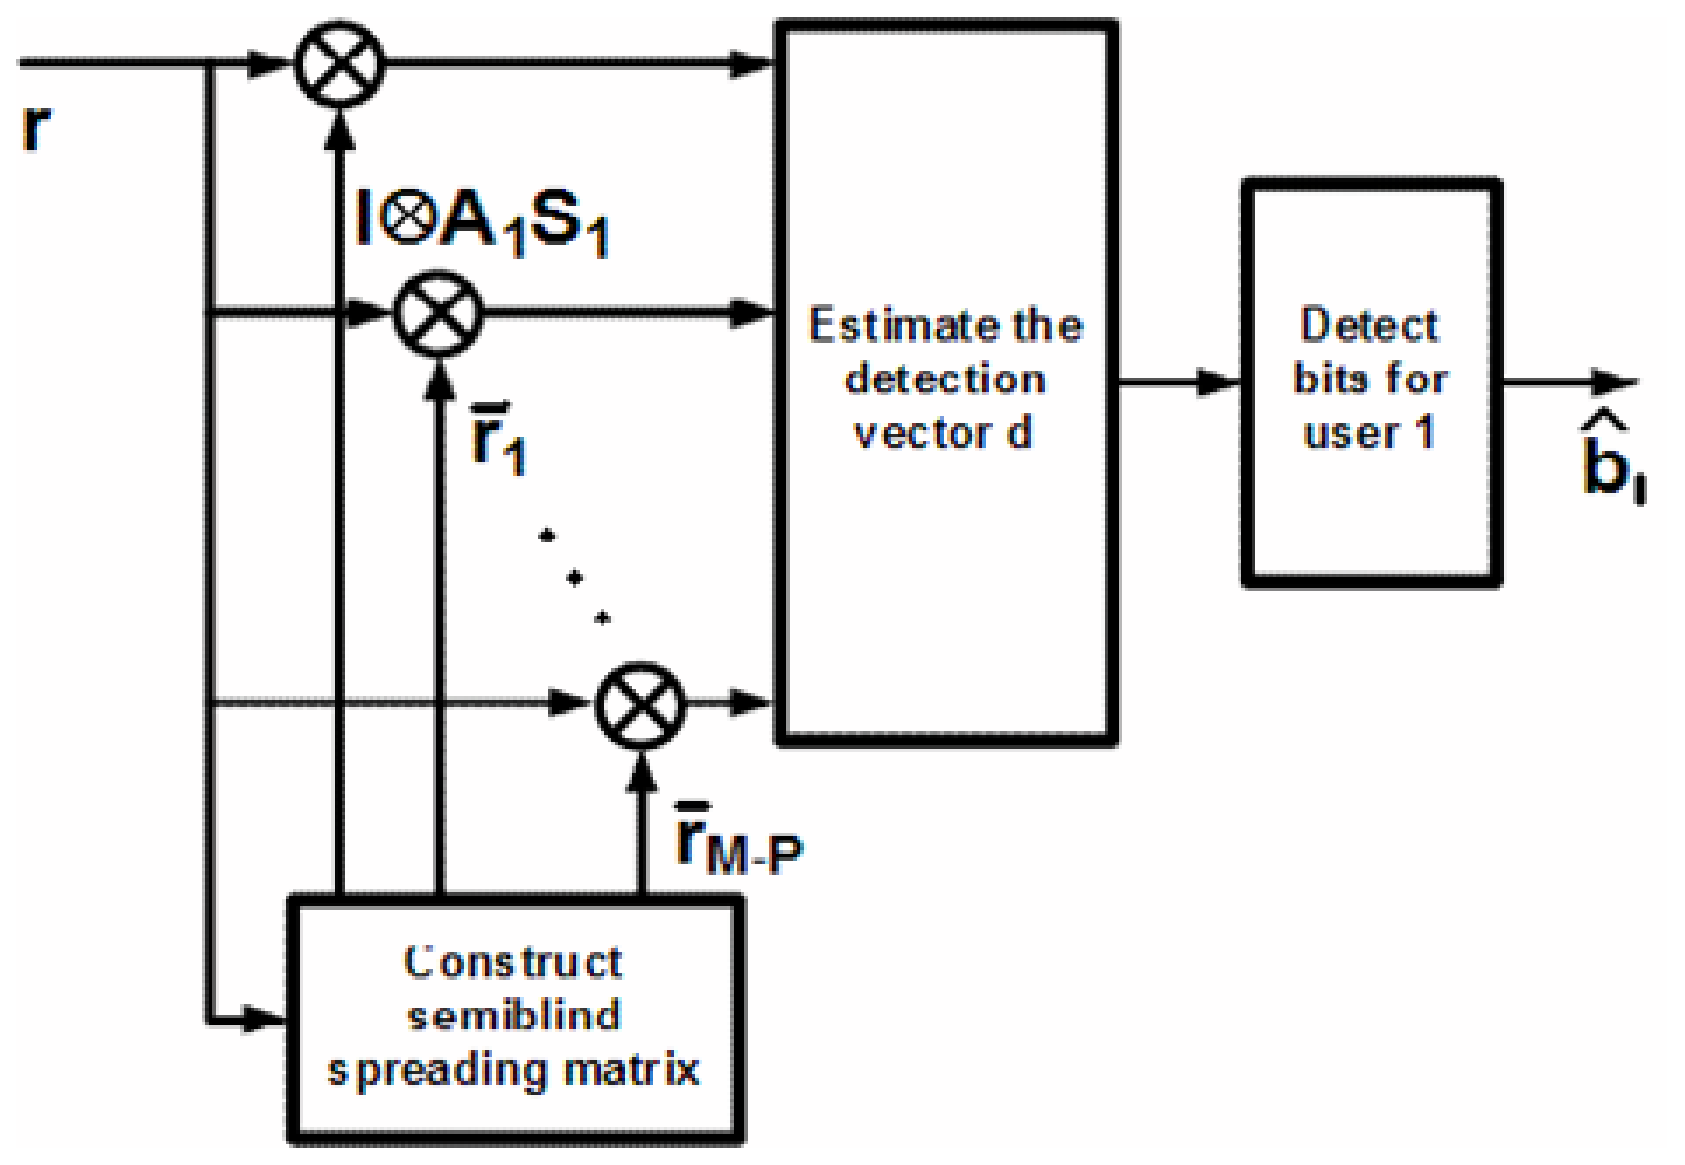
\includegraphics[width=2.5in]{SBMUDstruct2.eps}
\caption{The proposed semiblind Multiuser detection model and
framework. } }\label{MUD_model}
\end{figure}
\section{Semi-Blind Multiuser Detection}
After defining the known semi-blind signature matrix $\bcS$ in
(\ref{S}), the conventional signal model (\ref{r}) is transformed
into (\ref{rn}) with the desired bits vector $\bb_1$ replaced by
the detection vector $\bd$ and the original noise vector $\bn$
replaced by $\bar{\bn}$. On the other hand, the desired bits
vector $\bb$ can be detected using $\bd$, $\bG$ and
(\ref{bn_estimation}). Now the question is how to efficiently
estimate $\bd$ in (\ref{rn}). In the following, we develop new
estimation schemes based on LS, MUV and MMSE criteria.

\subsection{\em Least Square Estimation}

We first assume that the received measurements in $\bcS$ are
assumed to be free of error.  Hence, all errors are confined to
the received vector $\br$ due to $\bar\bn$ in (\ref{rn}) in the
$n$th bit interval.  The following LS estimator is proposed along
the lines of the classic decorrelating detector. Suppose $\bU^{\rm
T}\bcS\bV=\mathbf{\Sigma}$ is the SVD of
$\bcS\in\mathbb{R}^{PL\times
 M}$ with $r=\mbox{rank}\left\{\bcS\right\}$.  If $\bU=[\bu_1\ \bu_2\ \ldots\ \bu_{PL}]$,
 $\bV=[\bv_1\ \bv_2\ \ldots\ \bv_M]$, $\mathbf{\Sigma}={\rm diag}\{[\sigma_1\ \ldots\ \sigma_r\ 0\ \ldots\ 0]\}$ and $\br\in \mathbb{R}^{L\times 1}$, then~\cite{Golu96}
 \begin{equation}
 \matrix{\bd_{\rm LS} = \sum_{i=1}^{r} \frac{\bu_i^{\rm T}\br}{\sigma_i} \bv_i =
 \bcS^+\br}
 \label{LS}
 \end{equation}
minimizes $\|\bcS\bd-\br\|_2$ and has the smallest 2-norm of all
minimizers. Moreover, the minimum squared error achieved is
\begin{equation}
\varepsilon_{\rm
LS}^2=\min\limits_{\bx\in\mathbb{R}}\|\bcS\bx-\br\|_2^2=\sum\limits_{i=r+1}^{L}
\left(\bu_i^{\rm T}\br\right)^2 \enspace .
\end{equation}

so that the bit sent by the first user, $b_1$, in the $n$th
signaling interval is detected with
\begin{equation}
\begin{array}{rcl}
\hat{\bb}_{1\rm LS}&=&\mbox{sign}\left\{\bG^{\rm
T}\bcS^+\br\right\} \enspace .
\end{array} \label{b_LS}
\end{equation}

\subsection{\em Total Least-Square Estimation}

The previous LS estimate of the detection vector $\bd$ from
(\ref{rn}), (\ref{DetectorVector}) and (\ref{LS}) is the solution
to
\begin{equation}
\begin{array}{rcl}
\hat{\bd}=\matrix{\min\limits_{\bx}\left\|\br-\bcS\bx\right\|_2}&\mbox{subject
to}&\br\subseteq \mathbb{R}(\bcS)
\end{array}
\label{LSProb}
\end{equation}
where the semi-blind signature matrix $\bcS$ is assumed to be
error-free. However, this assumption is not entirely accurate
according to the definition of $\bcS$ in (\ref{S}) since there is
a noise term, $\bN$.

Furthermore, $\br$ can also be expressed as
\begin{equation}
\begin{array}{rcl}
\br&=&(\bcS-\bar\bN)\bB^{+}\bb + \bn\\
 &=&\hat{\bcS}\bd + \bar\bn
\end{array}
\end{equation}
where  $\hat{\bcS}=\bcS-\bN=\bS\bA\bB$.  The minimization problem
of (\ref{LSProb}) can then be transformed into the following TLS
problem:
\begin{equation}
\begin{array}{rcl}
\left[\hat{\bcS},\ \bx\right]&=&\matrix{\min\limits_{\bar{\bcS},\
\bx}\left\|\left[ \matrix{\bcS&\br} \right] - \left[
\matrix{\bar{\bcS}& \bar{\bcS}\bx}\right]\right\|_2}
\end{array},
\label{TLSProb}
\end{equation}
subject to $\br\subseteq\mathbb{R}(\bar{\bcS})$. Let
$\bcS=\bU^{'}\mathbf{\Sigma}^{'}\bV^{'T}$ and $[\bcS\
\br]=\bU\mathbf{\Sigma}\bV^{\rm T}$ be the SVD of $\bcS$ and
$[\bcS\ \br]$, respectively. If $\sigma_{PK+K-1}^{'}
> \sigma_{PK+K}$, then~\cite{Huff91}
\begin{equation}
\bd_{\rm TLS} = \left(\bcS^{\rm
T}\bcS-\sigma_{PK+K}^2\bI\right)^{-1}\bcS^{\rm T}\br
\end{equation}
and
\begin{equation}
\begin{array}{rcl}
\varepsilon_{\rm TLS}^{2}&=&\min\limits_{\bx\in
\mathbb{R}^{K\times
1}}\|\bcS\bx-\br\|_2^2 \\
 &=& \sigma_{PK+K}^2\left[1+\sum_{i+1}^{K}\frac{\left(\bu_i^{'T}\br\right)^2}
{\sigma_i^{'2}-\sigma_{PK+K}^2}\right]
\end{array}
\end{equation}
where $\bU=[\bu_1\ \bu_2\ \ldots\ \bu_{PL}]$, $\bV=[\bv_1\ \bv_2\
\ldots\ \bv_{M+1}]$, $\mathbf{\Sigma}={\rm diag}\{[\sigma_1\
\sigma_2 \ldots\ \sigma_{M+\min\limits\{PL-M,\ 1\}}]\}$ and
$\bU^{'}=[\bu_1^{'}\ \bu_2^{'}\ \ldots\ \bu_{PL}^{'}]$,
 $\bV^{'}=[\bv_1^{'}\ \bv_2^{'}\ \ldots\ \bv_{M}^{'}]$,
 $\mathbf{\Sigma}^{'}={\rm diag}\{[\sigma_1^{'}\ \sigma_2^{'}\ \ldots\ \sigma_M^{'}]\}$.

\noindent The bit sent by the first user, $b_1$, in the $n$th
signaling interval can be detected with
\begin{equation}
\begin{array}{rcl}
\hat{\bb}_{1\rm TLS}&=&\mbox{sign}\left\{ \bG\left(\bcS^{\rm
T}\bcS-\sigma_{PK+K}^2\bI\right)^{-1}
 \bcS^{\rm T}\br\right\} \enspace .
% &=&\mbox{sgn}\{b_n^1+[\matrix{A_1^{-1}&\bar{\bd}^{\rm T}}]\bcS^+\tilde{\bn}\}
\end{array}
\label{b_TLS}
\end{equation}

\subsection{\em Mixed LS/TLS Estimation}

In the LS problem of (\ref{LSProb}), it assumed the semi-blind
signature matrix $\bcS$ is error-free. Again, this assumption is
not completely accurate. In the TLS problem of (\ref{TLSProb}), it
assumed that in each column of the semi-blind signature matrix,
$\bcS$, some noise or error exists.  This assumption also is not
complete. Though there exists a noise or error matrix $\bN$ in
$\bcS$ from (\ref{S}), its first column is exactly known to be
noise-free or error-free.  Hence, to maximize the estimation
accuracy of the detection vector $\bd$, it is natural to require
that the corresponding columns of $\bcS$ be unperturbed since they
are known exactly. The problem  of estimating the detection vector
$\bd$ can then be transformed into the following MLS problem by
considering (\ref{LSProb}) and (\ref{TLSProb}):
\begin{equation}
\begin{array}{rcl}
\matrix{\min\limits_{\bar{\bcS},\
\bx}\left\|\left[\matrix{\tilde{\bcS}&\br}\right]-\left[\matrix{\bar{\bcS}&[\bA_1\bS_1\
 \bar{\bcS}]\bx}\right]\right\|_{2} }
\end{array}\label{MLSProb}
\end{equation}
subject to $\br\subseteq\mathbb{R}([\bA_1\bS_1\ \bar{\bcS}])$.
Consider the MLS problem in (\ref{MLSProb}) and perform the
Householder transformation $\bQ$ on the matrix
$[\matrix{\bcS&\br}]$ so that
\begin{equation}
\begin{array}{rcl}
\bQ^{\rm
T}[\matrix{\bA_1\bS_1&\bar{\bcS}&\br}]&=&\left[\matrix{\bR_{11}&\bR_{12}&R_{1r}\cr
\mathbf{0}&\bR_{22}&\bR_{2r}}\right]
\end{array}
\end{equation}
where $\bR_{12}$ is a $1\times (M-1)$ vector, $\bR_{22}$ is a
$(L-1)\times (M-1)$ matrix and $\bR_{2r}$ is a $(L-1)\times 1$
vector.

Denote $\sigma'$ as the smallest singular value of $\bR_{22}$ and
$\sigma$ as the smallest singular value of
$[\matrix{\bR_{22}&\bR_{2r}}]$. If $\sigma'>\sigma$, then the MLS
solution uniquely exists and is given by~\cite{Huff91}
\begin{equation}
\begin{array}{rcl}
\bd_{\rm MLS}&=&\left(\bcS^{\rm
T}\bcS-\sigma^2\left[\matrix{\bzero&\mathbf{0}\cr\mathbf{0}&\mathbf{I}_{M-1}}\right]\right)^{-1}\bcS^{\rm
T}\br
\end{array}.
\end{equation}

\noindent The bit sent by the first user, $b_1$, during the $n$th
signaling interval can be detected with
\begin{equation}\hspace{-0.01in}
\begin{array}{l}
\hat{\bb}_{1\rm MLS}=\mbox{sign}\left\{\bG\left(\bcS^{\rm
T}\bcS-\sigma^2\left[\matrix{\bzero&\mathbf{0}\cr\mathbf{0}&\mathbf{I}_{M-1}}\right]\right)^{-1}\bcS^{\rm
T}\br\right\}.
\end{array}\label{b_MLS}
\end{equation}

\subsection{\em Minimum Variance Unbiased Estimation}
The optimal estimator which constrains the bias to be zero and
minimizes the variance is termed MVU estimator. When MVU estimator
\begin{equation}
\begin{array}{rcl}
{\bd}_{\rm MVU}&=&{\bf f}(\br)
\end{array}
\end{equation}
exists, it may be found that it attains the Cramer-Rao Lower Bound
(CRLB) so that
\begin{equation}
\begin{array}{rcl}
\frac{\partial\ln Pr(\br;\ \bd)}{\partial\bd}&=&\bI(\bd)\left[{\bf
f}(\br)-\bd\right]
\end{array},
\end{equation}
\noindent where $Pr(\br;\ \bd)$ is the joint PDF of $\br$ and
$\bd$ and $\bI(\bd)$ is the Fisher information matrix (FIM)
defined by
\begin{equation}\hspace{-0.04in}
\begin{array}{rcl}
$\bI(\bd)$ &=& {\rm E} \left\{ \left( \frac{\partial \ln{Pr(\br;\
\bd)}}{\partial \bd} \right) \left( \frac{\partial \ln{Pr(\br;\
\bd)}}{\partial \bd} \right)^{\rm H} \right\}
\end{array}.
\end{equation}
\noindent Though the determination of the optimal MVU estimator is
generally difficult, it can be evident with linear constraint and
the MVU estimator for $\bd$ then is~\cite{Key93}
\begin{equation}
\begin{array}{rcl}
{\bbf}_{\rm MVU}&=&(\bcS^{\rm
T}\bC_{\bar{\bn}}^{-1}\bcS)^{-1}\bcS^{\rm
T}\bC_{\bar{\bn}}^{-1}\br\ .
\end{array} \label{BLUE}
\end{equation}
\noindent The covariance matrix of ${\bbf}_{\rm MVU}$ given by
\begin{equation}
\begin{array}{rcl}
{\bC}_{\bd_{\rm MVU}}&=&(\bcS^{\rm
T}\bC_{\bar{\bn}}^{-1}\bcS)^{-1}
\end{array}.
\end{equation}
\noindent Though the PDF of $\bB$ may be determined, the PDF of
$\bB^{+}$ is largely unknown. This makes it hard to calculate the
closed-form solution of $\bC_{\bd}$ and $\bC_{\tilde{\bn}}$.
However, with Girko's Law, when $\alpha=(PK+K-2)/(M-1)$ is fixed,
$K$, $M$ $\rightarrow\infty$, the diagonal element of
$\frac{1}{M-1}\tilde{\bD}^+\tilde{\bb}\tilde{\bb}^{\rm
T}\tilde{\bD}^{\rm +T}$ may be approximated
by~\cite{Muller,Hanly90}
\begin{equation}
\begin{array}{rcl}
\lim\limits_{k,M\leftarrow\infty}\frac{1}{M-1}\left[\tilde{\bD}^+\tilde{\bb}\tilde{\bb}^{\rm
T}\tilde{\bD}^{\rm +T}\right]_{ii}^{-1}&=&1-\alpha
\end{array}.
\end{equation}
\noindent Hence $\bC_{\bd}$ can be decided by
\begin{equation}
\begin{array}{rcl}
\bC_{\bd}&=&\left[\matrix{\frac{2M-PK-K}{M-PK-K+1}&\bzero^{\rm
T}\cr\bzero&\frac{1}{M-PK-K+1}\bI}\right]
\end{array},\label{d_var_new}
\end{equation}
\noindent and
\begin{equation}
\begin{array}{rcl}
\bC_{\bar\bn}&=&\sigma^{2}\frac{2M-PK-K}{M-PK-K+1}\bI
\end{array}\label{noise_var_new}
\end{equation}
\noindent and the bit vector for user $1$ can be detected by
\begin{equation}
\begin{array}{rcl}
\hat{\bb}_{1\rm MVU}&=&\mbox{sign}\left\{\bG(\bcS^{\rm
T}\bcS)^{-1}\bcS^{\rm T}\br\right\}
\end{array}\label{MVU_detector}
\end{equation}
\noindent Now we can see that the proposed MVU detector in
(\ref{MVU_detector}) actually has almost the same as the LS
detector proposed in~\cite{Wang03d,Wang03e}.

\subsection{\em Minimum Mean Squared Error Estimation}
Though the optimal Bayesian estimators are difficult to determine
in closed form or too computationally intensive to implement in
general, they can be found under the joint Gaussian assumption and
linear constrain. This class of MMSE estimators are generically
termed Wiener filter. Given measurements $\br$, the MMSE estimator
of $\bd$, ${\bd}_{\rm MMSE} = f( \br )$, minimizes the
mean-squared error $J_{\rm MSE}=E\{||\bd-\hat{\bd}||_2^2\}$. The
function $f(\br)$ may be nonlinear or linear and its exact
structure is determined by minimizing $J_{\rm MSE}$. When $\bbf$
and $\br$ are jointly Gaussian, the linear estimator $\bW_{\rm
MMSE}$ that minimizes the mean-squared error is (Bayesian
Gauss-Markov Theorem)
\begin{equation}
\begin{array}{rcl}
{\bd}_{\rm MMSE}&=&(\bC_{\bbf}^{-1}+\bcS^{\rm
T}\bC_{\bar{\bn}}^{-1}\bcS)^{-1}\bcS^{\rm
T}\bC_{\bar{\bn}}^{-1}\br
\end{array} \label{MSE}
\end{equation}
\noindent and its performance is measured by the covariance matrix
of the error ${\bf\epsilon}=\bd-\hat{\bd}$ given by
\begin{equation}\hspace{-0.0in}
\begin{array}{rcl}
\bC_{\bf\epsilon}&=&\left(\bC_{\bd}^{-1}+\bcS^{\rm
T}\bC_{\bar{\bn}}^{-1}\bcS\right)^{-1}
\end{array}.
\end{equation}
\noindent The bit vector for user $1$ can be detected by
\begin{equation}\hspace{-0.110in}
\begin{array}{l}
\hat{\bb}_1=\mbox{sign}\left\{\bG(\bC_{\bbf}^{-1}+\bcS^{\rm
T}\bC_{\bar{\bn}}^{-1}\bcS)^{-1}\bcS^{\rm
T}\bC_{\bar{\bn}}^{-1}\br\right\}\ .
\end{array}
\end{equation}
\noindent Combined with (\ref{d_var_new}) and
(\ref{noise_var_new}), $\hat{\bb}_1$ can be further simplified as
\begin{equation}\hspace{-0.0in}
\begin{array}{rcl}
\hat{\bb}_{1\rm MMSE}&=&\mbox{sign}\left\{\bG\left(\bf{\cal
C}\sigma^{2}+\bcS^{\rm T}\bcS\right)^{-1}\bcS^{\rm T}\br\right\}
\end{array}
\end{equation}
\noindent where
\begin{equation}
\begin{array}{rcl}
\bf{\cal C}&=&\left[\matrix{1&\bzero^{\rm
T}\cr\bzero&(2M-PK-K)\bI}\right]
\end{array}.
\end{equation}

\section{Adaptive Implementation}
Following the well-known Sherman-Morrison-Woodbury matrix inverse
lemma~\cite{Golu96}, an adaptive implementation of  the proposed
MVU semiblind detector can be expressed by
\begin{equation}\hspace{-0.0in}
\begin{array}{rcl}
\hat{\bb}_1(n)&=&\mbox{sign}\left\{\bG(n)\bcC_{\cal
S}^{+}(n)\bcS^{\rm T}(n)\br(n)\right\}
\end{array}
\end{equation}
\begin{equation}\hspace{-0.1in}
\begin{array}{l}
\bcC_{\cal S}^{+}(n)=\bcC_{\cal S}^{+}(n-1)-\bigl[\bcC_{\cal
S}^{+}(n-1)\bU(n-1)\bU^{\rm T}(n-1)\\
\hspace{0.2in}\bcC_{\cal S}^{+}(n-1)\bigr]\left[\bI+\bU^{\rm
T}(n-1)\bcC_{\cal S}^{+}(n-1)\bU(n-1)\right]^{-1}
\end{array}\label{adaptiveLS}
\end{equation}
\noindent where
\begin{equation}\hspace{-0.0in}
\begin{array}{rcl}
\bcC_{\cal S}(n)&=&\bcS(n)^{\rm T}\bcS(n)
\end{array}
\end{equation}
 \noindent and $\bU(n-1)$ is designed using SVD so that
\begin{equation}\hspace{-0.00in}
\begin{array}{rcl}
\bU(n-1)\bU^{\rm T}(n-1)&=&\bcC_{\cal S}(n)-\bcC_{\cal S}(n-1)
\end{array}
\end{equation}

\section{Performance Analysis}

\subsection{\em Multiuser Signal Model Comparison}
The comparison between the proposed asynchronous multiuser signal
models and the classic single-window signal model is given in
Table 1.
\begin{figure*}[t]\label{ModelComp}
\begin{center}
\begin{tabular}{lcc}
Parameters&The proposed model&The conventional model\\
\hline
Common/Shared& dedicated& shared\\
Required Timing Information&$\mbox{only user 1}$ & $\mbox{all users}$\\
Required Amplitude Information&$\mbox{only user 1}$ & $\mbox{all users}$\\
Required Spreading Sequences&$\mbox{only user 1}$ & $\mbox{all users}$\\
\hline
Input Vector&$\bf{r}\ -\ \rm 1\times\rm PL$&$\bf{r}_1\ -\ \rm 1\times\rm L$\\
Output Vector &$\bar\bb_1\ -\ 1\times\rm P$&$\bb_1\ -\ 1\times\rm K$\\
Num. of Detected Bits& P & 1\\
Spreading Matrix &$\bcS\ -\ \rm PL\times\rm M$&$\bS\ -\ \rm L\times\rm K$\\
Amplitude Matrix &$\rm N/A$&$\bf{A}\ -\ \rm K\times\rm K$\\
Noise Vector &$\bar\bn\ -\ 1\times\rm PL$&$\bn\ -\
1\times\rm L$\\
\hline
\end{tabular}
\end{center}
\center{Table 1. The comparison of the proposed semiblind
multiuser signal model and the conventional signal model}
\end{figure*}

\subsection{\em Comparison with The Classic Decorrelator}
When $P=1$, there is no noise in $\bcS$ and $\bG$ is accurately
known beforehand, there is the following relationship between the
user $1$'s MVU detector $\bw_{\rm MVU}$ and the decorrelator
$\bw_{\rm DD}$.
\begin{equation}
\begin{array}{rcccl}
\bw_{\rm MVU}&=&\bG(\bcS^{\rm T}\bcS)^{-1}\bcS^{\rm
T}&=&A_1^{-1}\bw_{\rm DD}
\end{array}
\end{equation} \label{wN0}
\noindent On the other hand, $\bw_{\rm DD}$ can be taken as a
special case of $\bw_{\rm BLU}$ with $\bB =\bI$ and $P=1$.

\subsection{\em The New Noise Vector $\bar{\bn}$}
The mean of the semi-blind noise term $\bar{\bn}$ in
(\ref{new_noise}) given by

\begin{equation}
\begin{array}{rcccl}
\bar{\bm}&=&{\rm E}\{\bar{\bn}\}&=&0
\end{array}
\end{equation}

\noindent The variance of $\tilde{\bn}$ satisfies the following
inequality

\begin{equation}\hspace{-0.0in}
\begin{array}{l}
\bigl|{\rm
E}\{(\bar{\bn}-\bar{\bm})^2\}\bigr|_{\infty}\leq\sigma_n^2+(P+1)(K-1)\|\tilde{\bD}^+\|_2^2\sigma_{\bar{n}}^2
\end{array} \label{noise_mean}
\end{equation}
\noindent where $\bigl|\star\bigr|_{\infty}$ denotes the infinity
norm of vector $\star$ and $\sigma_{\bar{n}}^2$ is the power of
the noise term $\bar{\bN}$ in the semi-blind signature matrix
$\bcS$.

\subsection{\em AME and Near-Far Resistance}
A commonly used performance measure for a multiuser detector is
AME and near-far resistance~\cite{Verd98}. Since the proposed
algorithms converge to the conventional decorrelating detector as
$\sigma\rightarrow 0$, their AME and near-far resistance for user
1 is
\begin{equation}
\begin{array}{rcccl}
\bar{\eta}_1&=&\left[\bR^{+}\right]_{11}^{-1}&=&\left[(\bS^{\rm
T}\bS)^{+}\right]_{11}^{-1}
\end{array}.
\end{equation}

\subsection{\em CRLB for $\bd$ Estimation}
The CRLB is given by the inverse of the FIM. Providing the blind
spreading matrix $\bcS$ is known beforehand, we first define the
parameter vector $\mathbf{\phi} = \left[\bar{\sigma}^{2}\
\bbf^{\rm T}\right]^{\rm T}$, where $\bar{\sigma}^{2}
=(1+\frac{M-1}{M-PK-K+1})\sigma^{2}$, for computing the FIM, which
is defined by
\begin{equation}
\begin{array}{rcl}
\bI(\mathbf{\phi}) &=& {\rm E} \left\{ \left( \frac{\partial
\ln{\rm Pr}}{\partial \mathbf{\phi}} \right) \left( \frac{\partial
\ln{\rm Pr}}{\partial \mathbf{\phi}} \right)^{\rm H} \right\}
\label{fim}
\end{array}
\end{equation}
\noindent where $\ln{\rm Pr}$ is the log-likelihood function given
by
\begin{equation}
\begin{array}{rcl}
\ln{\rm
Pr}&=&C-L\ln\bar{\sigma}^2-\frac{1}{2\bar{\sigma}^2}\parallel\mathbf{e}\parallel_2^2
\end{array},\label{logl}
\end{equation}
\noindent $C$ is a constant and $\mathbf{e}=\br-\bcS\bbf$.
Providing $\bcS$ is known, the closed-form CRLB expression of
$\bbf$ is then given by
\begin{equation}
\begin{array}{rcl}
{\rm CRLB}(\bbf\ |\ \bcS) &
=&(1+\frac{M-1}{M-PK-K+1})\sigma^{2}(\bcS^{\rm T}\bcS)^{\rm +}
\end{array}.\label{CRLB_f}
\end{equation}
\noindent From (\ref{CRLB_f}), it shows that the accuracy of
estimating $\bbf$ may increase with increasing $M$.
\section{Computer Simulations}
In this section, various computer simulation results are presented
to demonstrate the performance of our proposed semiblind
detectors. In our computer simulations, we assume a chip-level
synchronized single base station system. In this system, there are
$K=10$ users sending asynchronous signals to the base station. The
delays between interfering users and the first user are random
variables between $1$ and $63$ chips. All spreading sequences are
random sequences with the spreading gain $G=64$. The size of the
semiblind spreading matrix $\bcS$ is $64\times30$ with $M=30$.
\begin{figure} \center{
\includegraphics[width=2.5in]{BER_SNR3.eps}
\caption{The BER performance comparison of the single-user matched
filter, decorrelating detector and the proposed detectors. }
}\label{BER_SNR}
\end{figure}
In Fig. 2, we compare the BER performance of the proposed
semiblind detectors with the single-user matched filter (SU-MF)
and decorrelating detector against changing $SNR$. It shows that
the performance of the conventional decorrelator and SU-MF is
better than the proposed semiblind detectors when the near-far
ratio is small, $A_2/A_1=1.0$. However, when MAI is strong and
$A_2/A_1=10$, the SU-MF experiences the near-far problem and the
performance of the proposed semiblind detectors is between the
decorrelating detector and SU-MF.
\begin{figure} \center{
\includegraphics[width=2.5in]{BER_NFR4.eps}
\caption{The near-far resistance comparison of the single-user
matched filter, decorrelating detector and the proposed detectors.
$SNR=6dB$ } }\label{BER_NFR}
\end{figure}
In Fig. 3, we examine the near-far resistance of the proposed
semiblind detectors. We see that the near-far resistance of the
MVU detector is close to the decorrelating detector and the
near-far resistance of the MMSE semiblind detector is close to the
SU-MF when $A_2/A_1$ is small. When $A_2/A_1$ becomes large, the
near-far resistance of both the MVU and MMSE semiblind detectors
are close the SU-MF.
\begin{figure} \center{
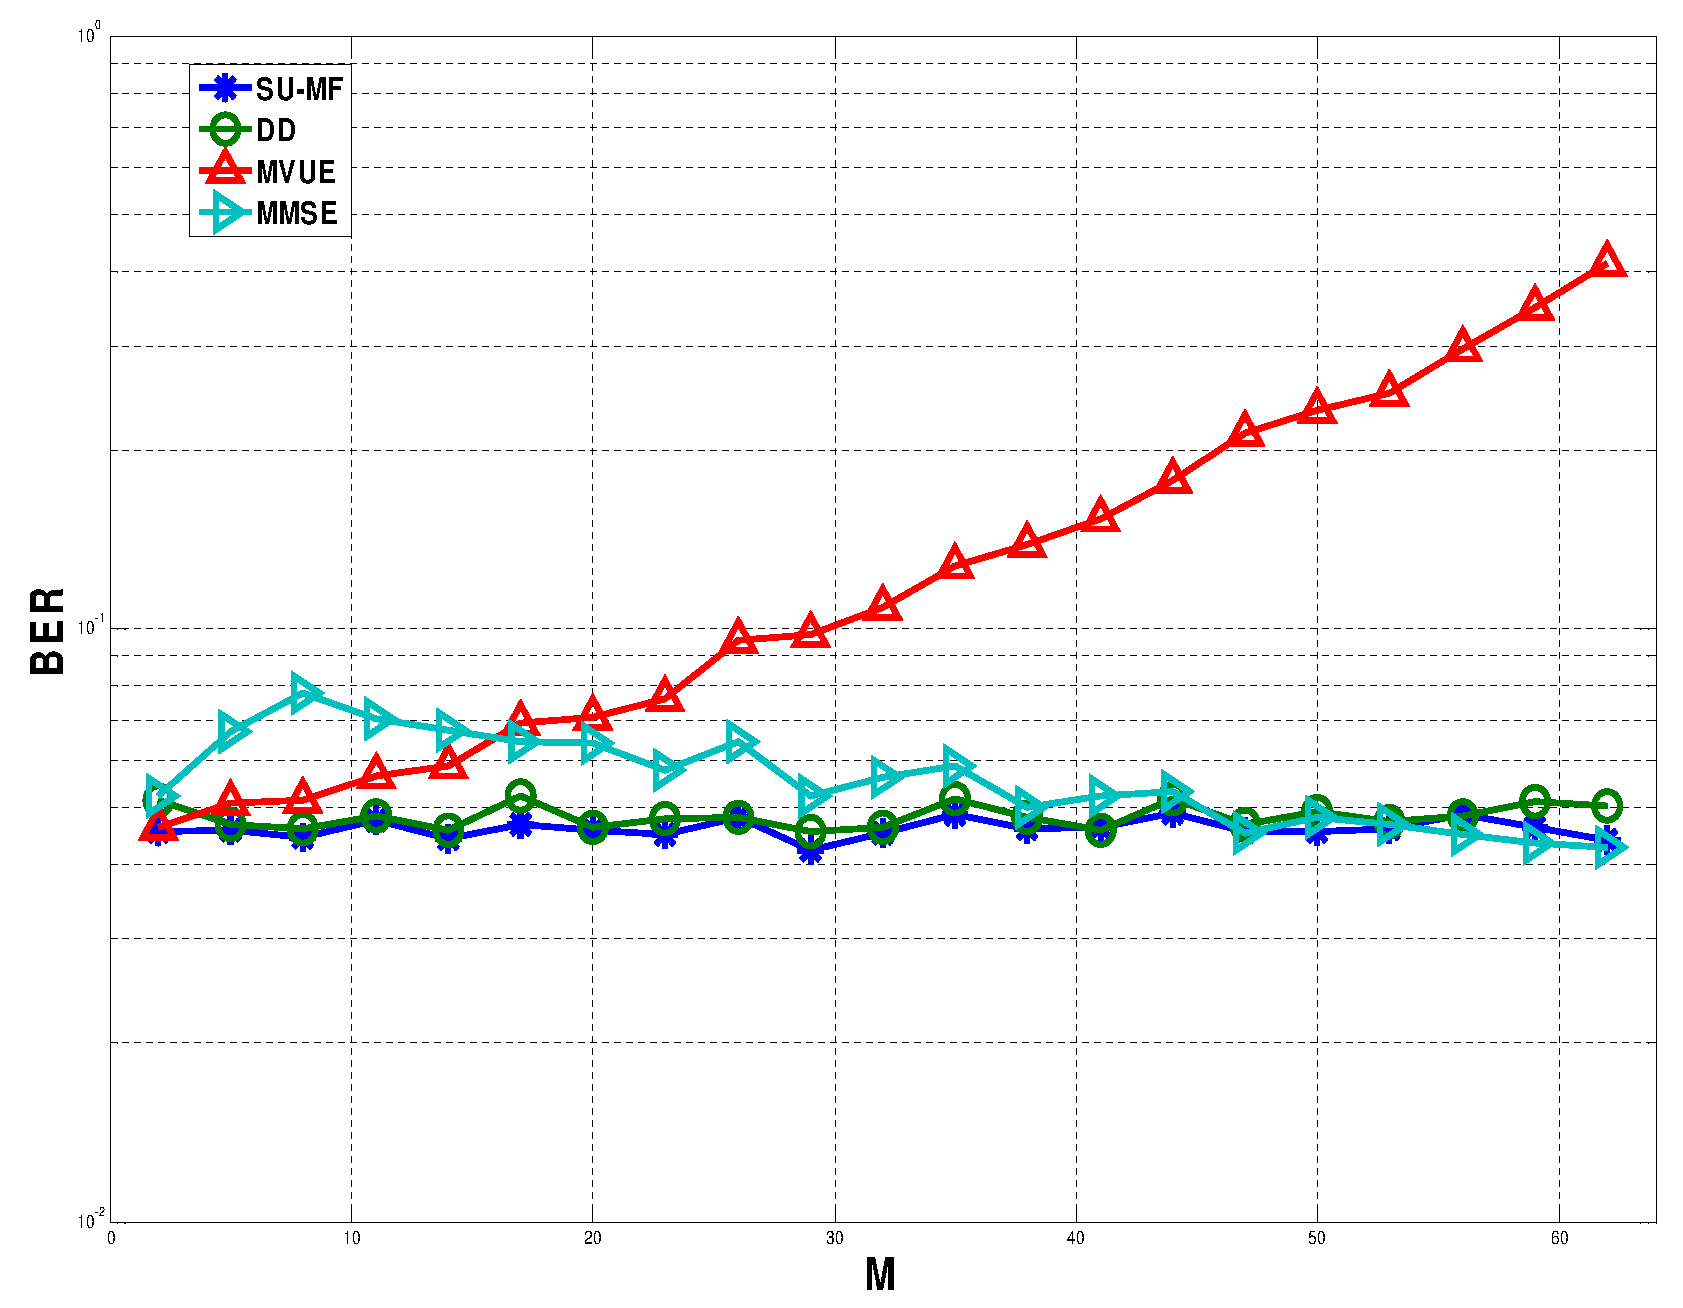
\includegraphics[width=2.5in]{BER_M2.eps}
\caption{The BER performance of the single-user matched filter,
decorrelating detector and the proposed detectors with changing
$M$. $P=1$ } }\label{BER_M}
\end{figure}
\begin{figure} \center{
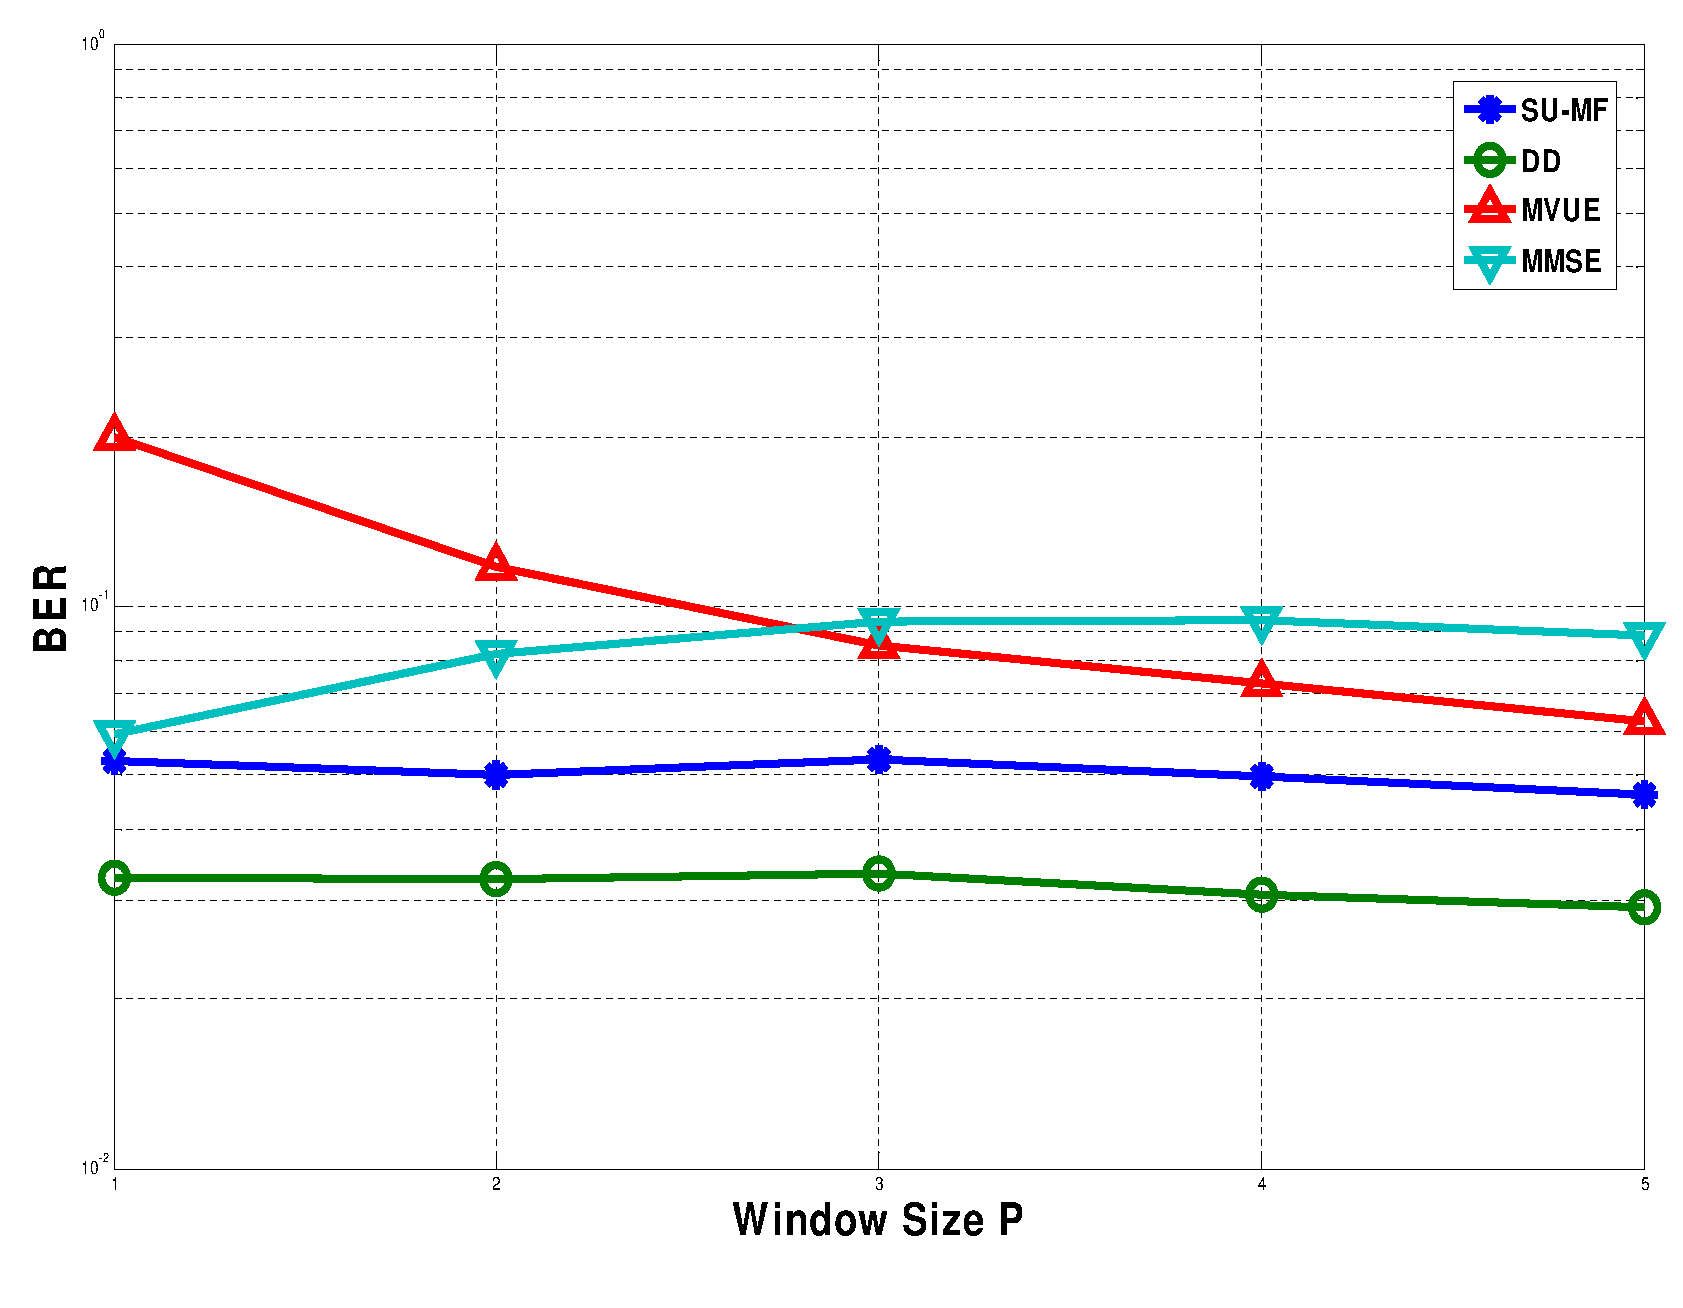
\includegraphics[width=2.5in]{BER_P2.eps}
\caption{The BER of the single-user matched filter, decorrelating
detector and the proposed detectors with changing $P$. $M=64$ }
}\label{BER_P}
\end{figure}
In Fig. 4 and 5, the BER performance of the proposed detectors is
compared with the conventional detectors with changing the $M$ and
$P$ individually. We see that the BER performance of the MVU
semiblind detector is going down and the BER performance of the
MMSE semiblind detector is going up when $M$ is increased.
However, the BER performance of the MMSE semiblind detector is
going down while the BER performance of the MVU detector is going
up when $P$ is increased.
\section{Conclusions}
In this paper, a new semiblind multiuser detection framework and
two semiblind detectors are proposed for asynchronous CDMA.
Compared with most existing semiblind/blind multiuser detection
schemes, the proposed schemes are simple and direct without any
estimation or subspace separation operation and require a minimum
number of previously received signals, as well as desired user's
spreading sequence, timing and amplitude. Their performance are
comparable with the conventional single-window decorrelating
detector.

\small
\bibliographystyle{unsrt}
\bibliography{J-AsynchSemiBlindDetector10}
\end{document}
